\documentclass[letter,12pt]{article}
\usepackage[utf8]{inputenc}
\usepackage{fullpage}
\usepackage{graphicx}
\usepackage{caption}
\usepackage{subcaption}
\usepackage{datetime}
\usepackage{indentfirst}
\usepackage{setspace}

\usepackage[backend=biber,maxbibnames=99,defernumbers=true]{biblatex}
	\addbibresource[datatype=bibtex]{Bibliography.bib}

\newdateformat{mydate}{\THEDAY\space \shortmonthname[\THEMONTH] \THEYEAR}

\title{Amateur Radio for Packet-Based Communication with Low Earth Orbit Satellites}
\author{Samuel Harkness}
\date{\mydate\today}

\begin{document}

\maketitle

\begin{abstract}
	The radiation tolerant computing team at Montana State University has received a grant to integrate a prototype computer system into an SSEL CubeSat.  In order to receive data from the orbiting system, information is packetized and sent down using the frequency spectrum reserved for Ham radio operators. This report will describe the history amateur radio, using packet technology on amateur radio, and describe the system used by SSEL.
\end{abstract}

\section{Background}	
	\subsection{Amateur Radio}
		Amateur radio began with the invention of the radio, so pinpointing the exact inventor of radio is difficult.  Notable contenders are Hertz, Tesla, and Marconi, but several others also lay claim to the title \cite{Bishop_05}.  The first amateur radio club, however is definitively known.  In 1908, students at Columbia University formed the Wireless Telegraph Club \cite{Sun_08}. Like many new technologies, radio operation at this stage was misunderstood by authorities, and basically operated in an unregulated fashion.
		
		This 'Wild West' of amateur radio came to an end after the sinking of the RMS \textit{Titanic}.  The \textit{Titanic} had 2 radio operators aboard, though neither were part of the crew.  Instead, John Phillips and Harold Bride were employees of Marconi, and were tasked with sending and receiving telegrams for passengers.  High-profile passengers kept the two so busy they ignored an ice warning from the \textit{Californian}, going so far as to transmit back, "Shut up!" Shipboard radios all operated at the same frequency for transmit and receive, and the courtesy warning was blocking the \textit{Titanic's} ability to communicate. \cite{Coughlan_12}
		
		Following inquiries into the sinking of the \textit{Titanic} \cite{Titanic_12}, the United States Congress passed the Radio Act of 1912 \cite{Radio_12}. This law restricted private stations to wavelengths of 200-10 meters, corresponding to frequencies of 1500 kHz - 30 MHz, commonly referred to as shortwave radio. Considered useless at the time, the number of radio hobbyists in the US sharply declined. It is also at this time the term 'ham' came to be synonymous with an amateur radio operator.  Ham is a slang term describing a sub-par actor, itself referencing the glut of sub-par actors for the titular role of the play \textit{Hamlet}.
		
		Early long distance radio services used surface wave propagation at very low frequencies (on the order of 3-30 kHz), but were unsuitable for anything but data because of the low data rates.  Very low frequency radios were certainly not capable of voice communication. They also required power-supplies on the order of several hundred kilowatts to provide sufficient signal strength to survive the attenuation of transmitting long distances.
		
		It was quickly discovered in the 1920s that shortwave radios, considered useless to commercial and government interests, were capable of long-range transmissions, with higher data rates, and orders of magnitude less power requirements. Shortwave radios utilize a phenomenon known as skywave propagation.  At a very basic level, amateur radio operators utilize the Earth's ionosphere to reflect radio waves around the curvature of the earth.  The surface of the Earth then reflects the wave back towards the ionosphere.  Losses at the reflection boundaries can remain quite small, enabling signals of only a few watts to cover the planet.  With a single reflection, distances of approximately 3500 kilometers can be reached. Multiple hops can cover continents and oceans. \cite{Rawer_93} In addition, the lower-altitude layers of the ionosphere largely disappear at night, which in turn leads to individual hops being longer. %Figure~\ref{skywave} is a simple rendering of skywave propagation.
		
		\begin{figure}[h!]
			\centering
			\includegraphics[width=.5\textwidth]{./PNGs/skywave.png}
			\caption{Radio waves reflecting off the ionosphere during skywave propagation \cite{Wiki_Skywave}}
			\label{skywave}
		\end{figure}
		
		However, not all of the signal is reflected by the ionosphere.  In fact, only a very small portion is reflected, while the rest is transmitted out into space.  This allows satellite communications, as well as even using the moon as a reflective surface. Figure~\ref{atmospheric_opactiy} shows that very little to none of the power in the ~5 cm to 10 m wavelengths is sorbed by the atmosphere.
		
		\begin{figure}[h!]
			\centering
			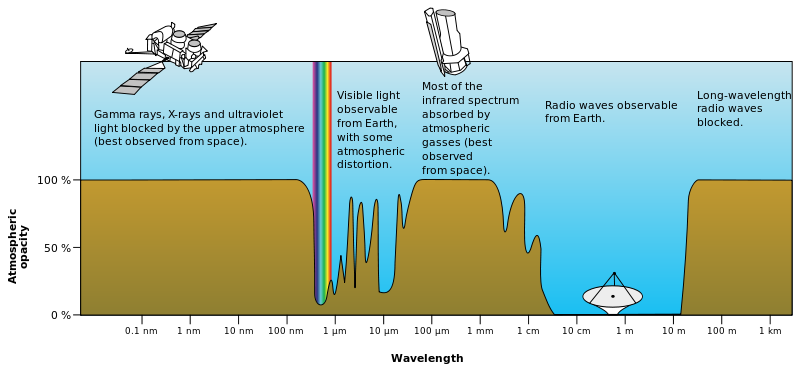
\includegraphics[width=\textwidth]{./PNGs/atmospheric_opacity.png}
			\caption{The opacity of Earth's atmosphere to the electromagnetic spectrum \cite{Wiki_Skywave}}
			\label{atmospheric_opactiy}
		\end{figure}		
		
		By 1924, communications as far as New Zealand to Great Britain were taking place.  This of course greatly interested the commercial sector, who wished to use it in place of expensive undersea cables.  Unfortunately, shortwave communication is plagued by noise, primarily from weather phenomena and other terrestrial causes, so commercial ventures were abandoned. Incidentally, Bell Labs was responsible for the birth of radio astronomy when they discovered a source of noise that seemed to appear four minutes earlier everyday than the previous, which turned out to be radio noise emitted from the center of the Milky Way. \cite{Finley_03}
		
		International connection between Hams prompted the first International Radiotelegraph Conference in Washington DC in 1927. At the conference, standard international radio bands of 80, 40, 20, and 10 meters wavelength were reserved for amateur use, as well as establishing radio callsign prefixes. \cite{Stewart_27} At the 1979 World Administrative Radio Conference (WARC) in Geneva, Switzerland, the 30, 17, and 12 meter bands were established for amateur radio use.  These bands are commonly referred to as the WARC bands. In the US today, Amateur radio comprises 16 different bands, ranging from 160 meters down to 23 centimeters. Figure~\ref{ARRL_Chart} graphically shows the US Amateur Spectrum.
		
		\begin{figure}[h!]
			\centering
			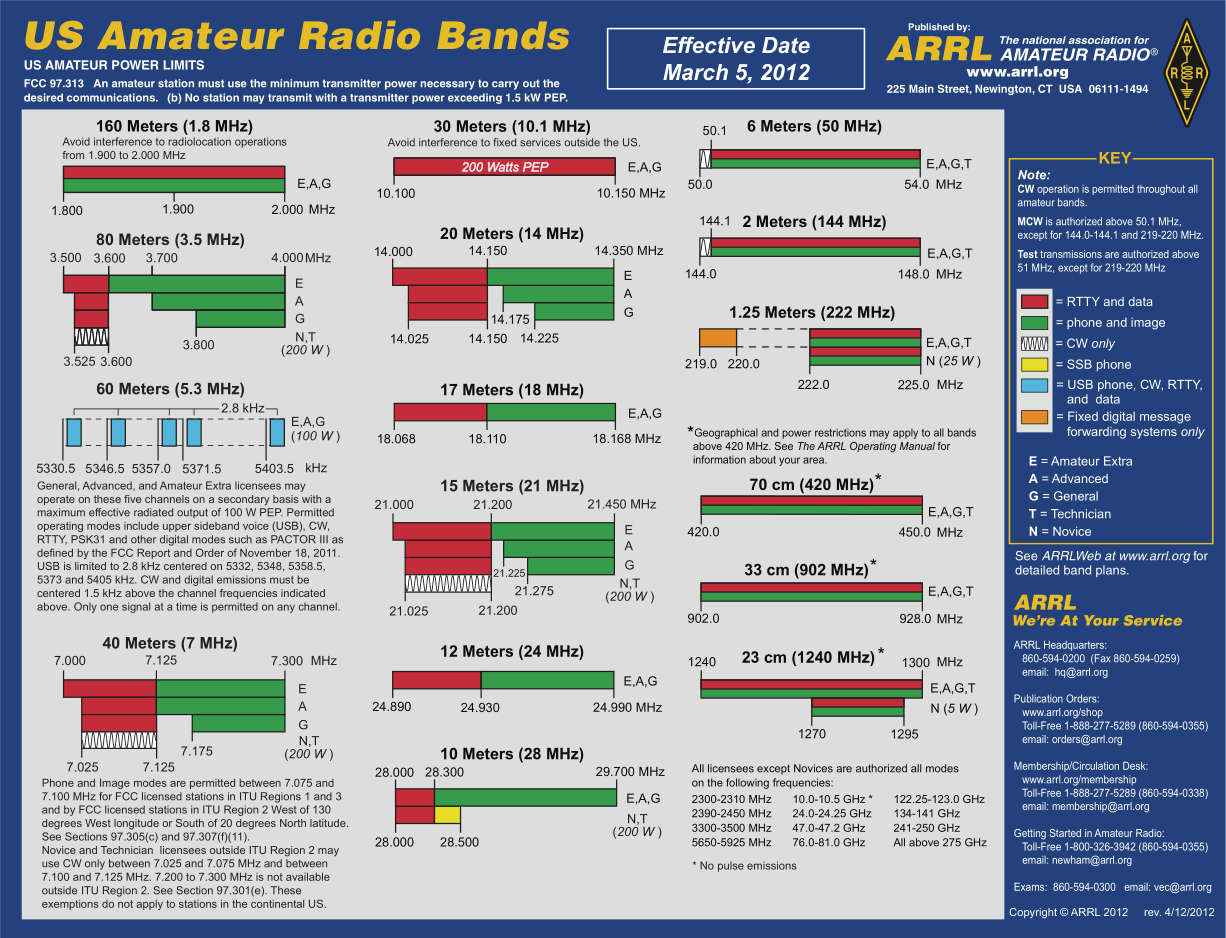
\includegraphics[width=\textwidth]{./PNGs/Amateur_Spectrum.png}
			\caption{US Amateur Radio Bands \cite{ARRL_Chart}}
			\label{ARRL_Chart}
		\end{figure}
		
	\subsection{Packets on Amateur Radio}
		Because radios inherently share a broadcast medium (the radio spectrum), access control was a great hurdle to implementing packet-based protocols on radios.  ALOHAnet was deployed in June 1971 at the University of Hawaii. \cite{Schwartz_09} The goal of ALOHAnet was to connect users on Oahu and the other Hawaiian islands with a central time-sharing computer on the main Oahu campus.  
		
		The original ALOHA protocol was full-duplex, using two distinct frequencies, in a hub configuration.  To equate it to modern Ethernet, the central node was a hub while all other nodes were workstations.  ALOHA did not contain any provisions for collision avoidance, instead relying on acknowledgments from the hub to detect collisions and retransmit packets. Further refinements to ALOHA lead to Carrier Sense Multiple Access protocols, such as Ethernet. \cite{Binder_75}
		
		Following DARPA's research into packet radio networks, Hank Magnuski had the foresight to obtain an allocation of Internet addresses for the use of amateur radio experimenters, commonly referred to as AMPRNet (AMateur Packet Radio Network). Within regional communities, amateur operators communicate with each by radio.  In order to connect these regional communities together, volunteers have set up a series of gateways and IP tunnels through the Internet.  These tunnels provide a mechanism for transporting AMPRNet IP packets across the Internet as though there were a radio link between the two tunnel endpoints. Traditionally the tunnels are connected via static tables updated by the same volunteers, but recent experimentation has moved to dynamic configurations provided by Peer to Peer VPN. \cite{Kantor_11}
	
		As of July 2011, there are more than 250 blocks of addresses allocated to more than 140 countries. Thousands of addresses have been assigned to hams around the world.  There have been more than 50 tunnel gateways registered, with more than 90 in operation. \cite{Kantor_11}
		
	\subsection{Amateur Radio on Satellites}
		The majority of artificial satellites have been and are in Low Earth Orbit (LEO). LEO is an orbit between the atmosphere and below the inner Van Allen radiation belt.  Altitudes are between 160 kilometers and 2,000 km, though altitudes less than 300 km experience large atmospheric drag.  Satellites complete a complete revolution around Earth anywhere from 88 minutes to 127 minutes.
		
		The first amateur satellite, OSCAR 1 (Orbiting Satellite Carrying Amateur Radio), launched on 12 December 1961, barely four years after Sputnik 1. The satellite had to meet very specific design specifications as it was used to replace one of the balance weights in the rocket stage. It also could not contain any propulsions system so as not to pose danger to the primary payload of the launch.  Despite being in orbit for only 22 days, OSCAR 1 as an immediate success with over 570 amateur radio operators in 28 countries connecting. Over the 50 years since the launch of OSCAR 1, more than 70 other amateur radio satellites have been put into orbit. \cite{RadioSatellites_06}
		
		
	
\section{SSEL Radio System}
	\subsection{Radio}
		The radio SSEL uses for satellite communications is the AstroDev He-100, depicted in Figure~\ref{fig:He-100}. The He-100 uses Gaussian minimum Shift Keying (GMSK), which has the advantage of reducing sideband power, which in turn reduces out-of-band interference between signal carriers in adjacent frequency channels. GMSK has high spectral efficiency, but it needs a higher power level in order to reliably transmit the data. \cite{Wiki_MSK}
		
		\begin{figure}[h!]
			\centering
			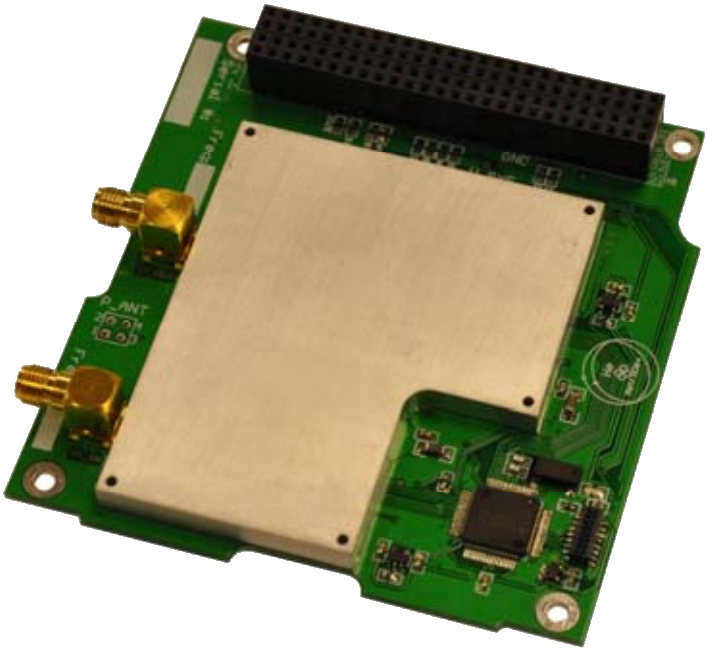
\includegraphics[width=.6\textwidth]{./PNGs/He-100_Radio.png}
			\caption{AstroDev He-100 \cite{He-100_Manual}}
			\label{fig:He-100}			
		\end{figure}
		
		The frequencies SSEL satellites communicate over vary slightly mission-to-mission as spectrum allocations must be coordinated with the International Amateur Radio Union and the FCC.  Downlink frequencies are typically around 437.00 MHz, while uplink frequencies are around 145.800 MHz.		
		
		Due to the high speed of orbital satellites, the uplink and downlink frequencies will vary during the course of a satellite pass.  This phenomenon is known as the Doppler effect.  While the satellite is moving towards the ground station, the downlink frequency will appear to be higher than normal, so the ground station receiver must be adjusted higher to continue receiving.  In turn, the satellite will be receiving the uplink signal at a higher frequency than the ground station is transmitting, so the ground station must transmit at a lower frequency in order maintain communications. After the satellite passes overhead and is moving away from the ground station, the process reverses itself. Figure~\ref{doppler_effect} shows the Doppler effect for a radio source moving to the right. Thankfully, software is designed and programmed to account and correct for the Doppler effect.
		
		\begin{figure}[h!]
			\centering
			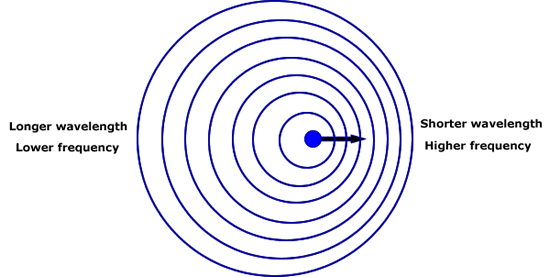
\includegraphics[width=\textwidth]{./PNGs/doppler_effect.png}
			\caption{Doppler Effect}
			\label{doppler_effect}			
		\end{figure}
		
		The following mathematical formulas relate the Doppler shift to the velocity of the satellite.
		
		\begin{center}
		\begin{tabular}{c c c}
			\textbf{Change in Frequency} & \textbf{Downlink Correction} & \textbf{Uplink Correction} \\
			\Large{$\Delta f = f \times \frac{v}{c}$} & \Large{$f_d = f(1 + \frac{v}{c})$} & \Large{$f_u = f(1 - \frac{v}{c})$} \\
		\end{tabular}
		\end{center}
		
		SSEL operates the He-100 radio in two different modes: Beacon and Downlink.  In normal operation, the spacecraft is in beacon mode where it beacons 214 bytes of data (not including the AX.25 overhead) every 60 seconds at 9600 bps.  The beacon period is directly impacted by power constraints; that is if there is more power available, data can be sent down with a smaller period separating beacons.  From the ground station, the spacecraft can be commanded to enter downlink mode, in which the AstroDev downlinks 231 byte packets at 19200 bps.  Because of link margins, downlink mode can only operate from approximately 20$^\circ$ above the horizon, or 140$^\circ$  of the sky.  This amounts to approximately 5 minutes of downlink time per pass. Figures~\ref{fig:Beacon} and \ref{fig:Downlink} show the Spectrums for Beacon and Downlink modes respectively.
		
		\begin{figure}[h!]
			\centering
			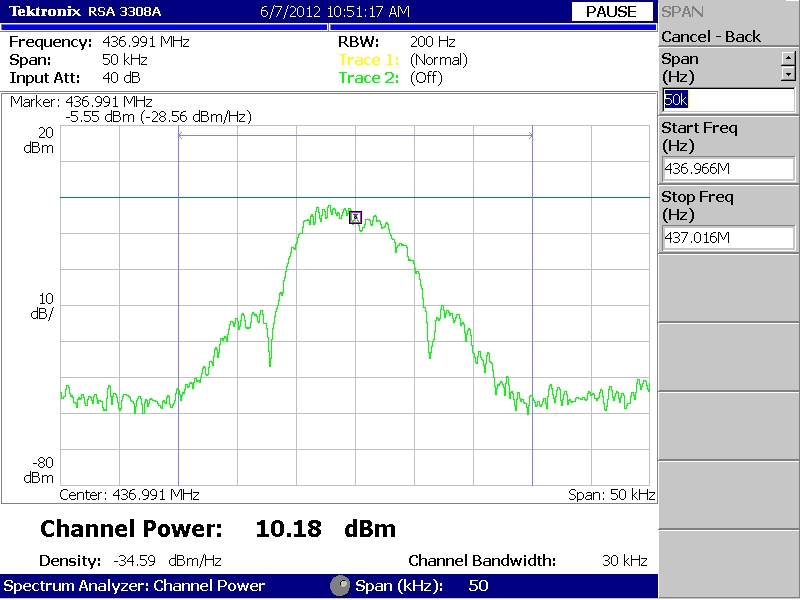
\includegraphics[width=\textwidth]{./PNGs/Beacon_50k_span_9600.png}
			\caption{Beacon Mode Spectrum}
			\label{fig:Beacon}			
		\end{figure}
		
		\begin{figure}[h!]
			\centering
			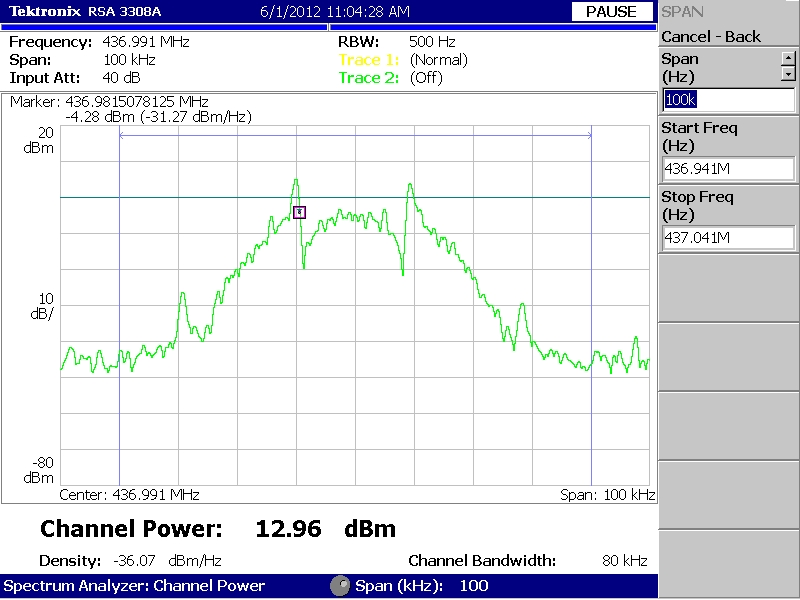
\includegraphics[width=\textwidth]{./PNGs/Downlink_100k_span_19200.png}
			\caption{Downlink Mode Spectrum}
			\label{fig:Downlink}			
		\end{figure}			
		
	\subsection{AX.25}
		AX.25 is a data link layer (OSI Layer 2) protocol derived from the X.25 protocol suite and designed for use with amateur radios. Figure~\ref{fig:AX25_Protocol_Stack} shows the protocol stack for AX.25. AX.25 can also perform the functions of a network layer (OSI Layer 3) protocol. AX.25 can operate in a connectionless or connection-oriented manner. \cite{Beech_98}
	
		\begin{figure}[h!]
			\centering
			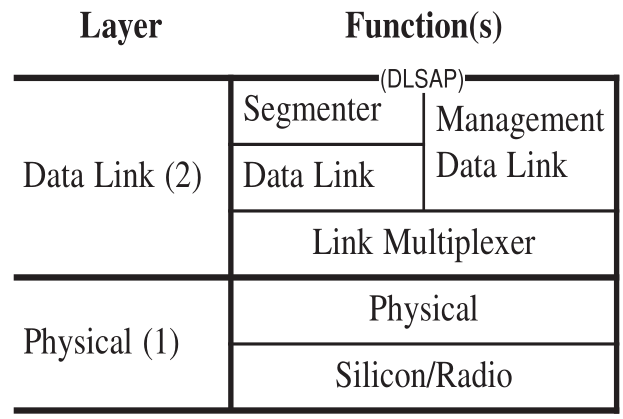
\includegraphics[width=.5\textwidth]{./PNGs/AX25_Protocol_Stack.png}
			\caption{AX.25 Protocol Stack \cite{Beech_98}}
			\label{fig:AX25_Protocol_Stack}			
		\end{figure}
		
		There are three general types of AX.25 frames: 
		\begin{itemize}
			\item Information frame (I frame)
			\item Supervisory frame (S frame)
			\item Unnumbered frame (U frame)
		\end{itemize}
		As can be seen in Figure~\ref{fig:AX25_Frame}, AX.25 frames are multiples of 8-bits, so can be measured in bytes. 
		
		\begin{figure}
			\centering
			\begin{subfigure}[b]{\textwidth}
				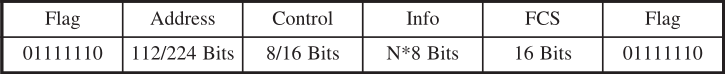
\includegraphics[width=\textwidth]{./PNGs/AX25_US_Frame.png}
				\caption{U and S frame construction}
				\label{fig:AX25_US_Frame}
			\end{subfigure}
			
			\vspace{12pt}
			
			\begin{subfigure}[b]{\textwidth}
				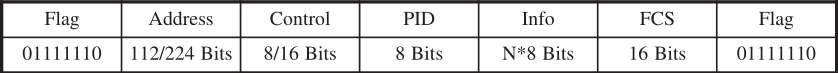
\includegraphics[width=\textwidth]{./PNGs/AX25_Information_Frame.png}
				\caption{I frame construction}
				\label{fig:AX25_I_Frame}
			\end{subfigure}
			
			\caption{AX.25 Frame Construction \cite{Beech_98}}
			\label{fig:AX25_Frame}
		\end{figure}
	
		AX.25 frames are broken down into distinct fields.
		\begin{itemize}
			\item The flag field uses the same symbol for both the start and stop symbol.  Two frames may share one flag, which would denote the end of the first frame and the start of the next frame.  In order to ensure that the flag bit sequence mentioned above does not appear accidentally anywhere else in a frame, the sending station monitors the bitstream for 5 contiguous logical 1 bits.  Any time the patter is sent, the sending station inserts a logical 0 after the fifth 1.  During frame reception, any time five contiguous logical 1s are received, a 0 bit immediately following the pattern is discarded.
			\item The address field identifies both the source and destination addresses. 
			\item The control field identifies the type of frame being passed (i.e. I,S,U) and controls several attributes of the Layer 2 connection.
			\item The Protocol Identifier (PID) field identifies which kind of Layer 3 protocol, if any, is used. Figure~\ref{fig:AX25_PID_Definitions} shows the encoding of the PID field.
			\item The information (I) field is the encapsulated packet from a higher layer protocol.  The I field defaults to 256 octets (bytes).
			\item The Frame-Check Sequence (FCS) is a 2-byte forward error correction. The FCS is calculated in accordance with ISO 3309.
		\end{itemize}
		
		\begin{figure}[h!]
			\centering
			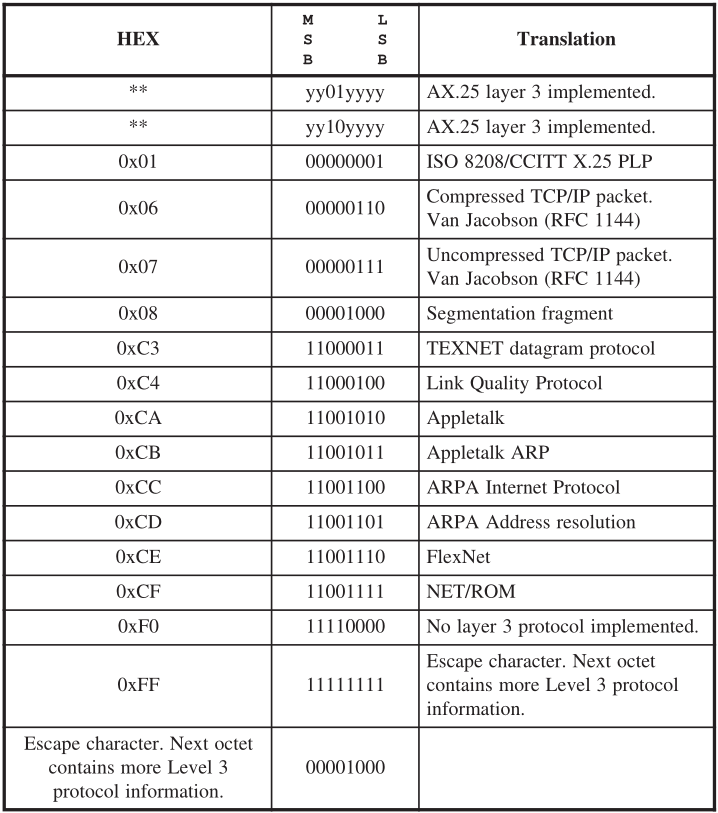
\includegraphics[width=.7\textwidth]{./PNGs/AX25_PID_Definitions.png}
			\caption{PID Definitions \cite{Beech_98}}
			\label{fig:AX25_PID_Definitions}			
		\end{figure}
		
		One area where SSEL deviates from the AX.25 standard is in the size of the information field.  The data packet can be no greater than 231 bytes.  This is due to the limitations with sending data to the AstroDev He-100 radio, as it will start to hang if the data field is any larger. The He-100 Manual states packets must be less than 255 bytes, but SSEL has modified the requirement through extensive testing. \cite{He-100_Manual}
		
\section{Conclusion}
	Amateur radio, packet technology, and satellite communications have evolved alongside each other since their invention.  Amateur radio operators were responsible for some of the earliest advances in packet technology. Hams have also been involved with satellite communications since their inception. These technologies are all intertwined, and will like depend on each other into the future.
		
\pagebreak		
\printbibliography
		
\end{document}